\documentclass[letterpaper]{article}

%% Language and font encodings
\usepackage[english]{babel}
\usepackage[utf8x]{inputenc}
\usepackage[T1]{fontenc}

%% Sets page size and margins
\usepackage[letterpaper,top=3cm,bottom=2cm,left=2cm,right=2cm,marginparwidth=1.75cm]{geometry}

%% Useful packages
\usepackage{amsmath}
\usepackage{graphicx}
\usepackage[colorinlistoftodos]{todonotes}
\usepackage[colorlinks=true, allcolors=blue]{hyperref}
\usepackage{mathtools}
\usepackage{latexsym}

\usepackage{tikz}
\usetikzlibrary{automata,positioning}

\title{Speech Processing HW 4}
\author{Matt Ruffner}

\begin{document}
\maketitle

\section{}

$A=[
\begin{bmatrix}
    
\end{bmatrix}$


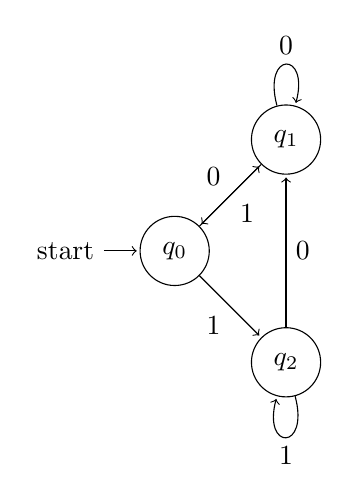
\begin{tikzpicture}[shorten >=1pt,node distance=2cm,on grid,auto] 
   \node[state,initial] (q_0)   {$q_0$}; 
   \node[state] (q_1) [above right=of q_0] {$q_1$}; 
   \node[state] (q_2) [below right=of q_0] {$q_2$}; 
    \path[->] 
    (q_0) edge  node {0} (q_1)
          edge  node [swap] {1} (q_2)
    (q_1) edge  node  {1} (q_0)
          edge [loop above] node {0} ()
    (q_2) edge  node [swap] {0} (q_1) 
          edge [loop below] node {1} ();
\end{tikzpicture}



\end{document}